\section{Parameter Efficiency with CNNs}

\subsection{CNN Implementation}

\subsubsection{Recorded Values}
\begin{itemize}
    \item Final validation accuracy: \textbf{99.03\%}
    \item Number of parameters: \textbf{421,642}
    \item Training time: \textbf{4.8 minutes}
    \item Number of epochs: \textbf{20}
\end{itemize}

\begin{figure}[h]
    \centering
    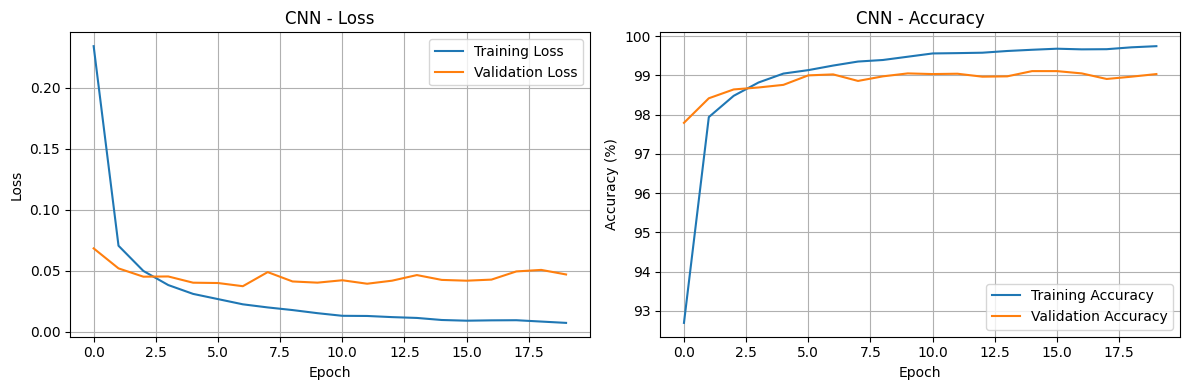
\includegraphics[width=0.8\linewidth]{section3/cnn.png}
    \caption{Training and validation curves for CNN model}
    \label{fig:cnn}
\end{figure}

\subsection{Efficiency Analysis}

\subsubsection{Question 3.1: Parameter Comparison}

The CNN has significantly fewer parameters than the MLP:

\begin{table}[h]
\centering
\begin{tabular}{|l|c|c|}
\hline
\textbf{Model} & \textbf{Parameters} & \textbf{Reduction} \\ \hline
MLP (Baseline) & 535,818             & ---                \\ \hline
CNN            & 421,642             & 114,176 (21.3\%)   \\ \hline
\end{tabular}
\caption{Parameter count comparison between MLP and CNN}
\label{tab:cnn-parameters}
\end{table}

The CNN achieves a 21.3\% reduction in parameters compared to the baseline MLP, demonstrating superior parameter efficiency through the use of convolutional layers with weight sharing instead of fully-connected layers.

\subsubsection{Question 3.2: Accuracy Comparison and CNN Suitability}

Despite having 114,176 fewer parameters, the CNN achieves superior validation accuracy compared to all MLP variants:

\begin{table}[h]
\centering
\begin{tabular}{|l|c|c|c|}
\hline
\textbf{Model}        & \textbf{Parameters} & \textbf{Val Accuracy} & \textbf{Train-Val Gap} \\ \hline
MLP (Baseline)        & 535,818             & 97.74\%               & 2.05\%                 \\ \hline
MLP (Dropout)         & 535,818             & 98.31\%               & 1.08\%                 \\ \hline
MLP (Early Stopping)  & 535,818             & 97.90\%               & 1.66\%                 \\ \hline
\textbf{CNN}          & \textbf{421,642}    & \textbf{99.03\%}      & \textbf{0.77\%}        \\ \hline
\end{tabular}
\caption{Performance comparison: CNN vs MLP variants}
\label{tab:cnn-performance}
\end{table}

The CNN outperforms the best MLP (dropout) by 0.72\% in validation accuracy while using 21.3\% fewer parameters. This demonstrates that CNNs are fundamentally better suited for image data for several reasons:

\begin{enumerate}
    \item \textbf{Spatial structure preservation}: Convolutional layers process local regions of pixels, maintaining the 2D spatial relationships that are crucial for image understanding. In contrast, MLPs flatten images into 1D vectors, destroying spatial information.
    
    \item \textbf{Hierarchical feature learning}: CNNs learn features in a hierarchical manner---early convolutional layers detect low-level features like edges and corners, middle layers combine these into textures and parts, and deeper layers recognize complete objects. This mimics the human visual system.
    
    \item \textbf{Translation invariance}: Through weight sharing, the same convolutional filters are applied across the entire image, allowing the network to recognize patterns regardless of their position in the image. A digit in the top-left corner is recognized as easily as one in the bottom-right.
    
    \item \textbf{Parameter efficiency}: Convolutional layers share weights across spatial locations, dramatically reducing the number of parameters compared to fully-connected layers while maintaining representational power. For example, a 3$\times$3 convolutional filter with 32 channels requires only 288 parameters, whereas a fully-connected layer connecting a 28$\times$28 image to 32 outputs would require 25,088 parameters.
\end{enumerate}

\subsection{Overfitting Analysis}

The CNN exhibits minimal overfitting compared to the baseline MLP:

\begin{itemize}
    \item \textbf{Loss curves}: Training and validation loss curves remain close together throughout training. Validation loss stabilizes around 0.04--0.05 without the divergence observed in the baseline MLP.
    
    \item \textbf{Train-validation gap}: The gap between training accuracy (99.8\%) and validation accuracy (99.03\%) is only 0.77\%, compared to 2.05\% in the baseline MLP. This indicates excellent generalization.
    
    \item \textbf{Training efficiency}: The CNN required only 20 epochs to achieve superior performance, compared to 50 epochs for the MLP, demonstrating faster convergence.
\end{itemize}

\subsection{Conclusion}

The CNN demonstrates clear superiority over MLP architectures for image classification tasks. With 21.3\% fewer parameters, it achieves 99.03\% validation accuracy---the highest among all tested models---while exhibiting minimal overfitting (0.77\% train-val gap). 

The convolutional architecture's ability to preserve spatial information, learn hierarchical features, and achieve translation invariance through weight sharing makes it fundamentally more suitable for image data than fully-connected networks. This experiment confirms why CNNs have become the standard architecture for computer vision tasks, offering both better performance and greater parameter efficiency.